Consider the following hamiltonian for a spin-1/2 particle.

\begin{equation}\label{eq:spin-half}
    H = \vec{S} \cdot \vec{\sigma} = \begin{pmatrix}
        \cos\theta & \sin\theta e^{i\phi} \\ 
        \sin\theta e^{i\phi} & -\cos\theta    
    \end{pmatrix}
\end{equation}

where $S \equiv (\cos\phi\sin\theta, \sin\phi\sin\theta, \cos\theta)$ is a classical spin with $|S| = 1$. 
\vspace{0.5cm}\\
It is easily seen that the hamiltonian can be diagonalized by the following unitary matrix.
\begin{equation}\label{eq:rot}
    U = \begin{pmatrix}
        \cos\frac{\theta}{2} & -\sin\frac{\theta}{2}e^{-i\phi} \\ 
        \sin\frac{\theta}{2}e^{i\phi} & \cos\frac{\theta}{2}
    \end{pmatrix}
\end{equation}
Generally such a matrix is only unique upto a permutation and scaling of the columns. We would like to find a simple scheme to find such a matrix for systems with spin $>$ 1/2 without having to compute the eigenvectors first. Thinking about this procedure from a different perspective, we simply want to find a matrix that rotates the spin quantization axis from $\hat{z}$ to align with $\vec{S}$.

%%% FIG %%%
\begin{figure}[!htb]
    \centering
    \begin{subfigure}[b]{\textwidth}  %keep total sum <1 to show in same line
        \centering
        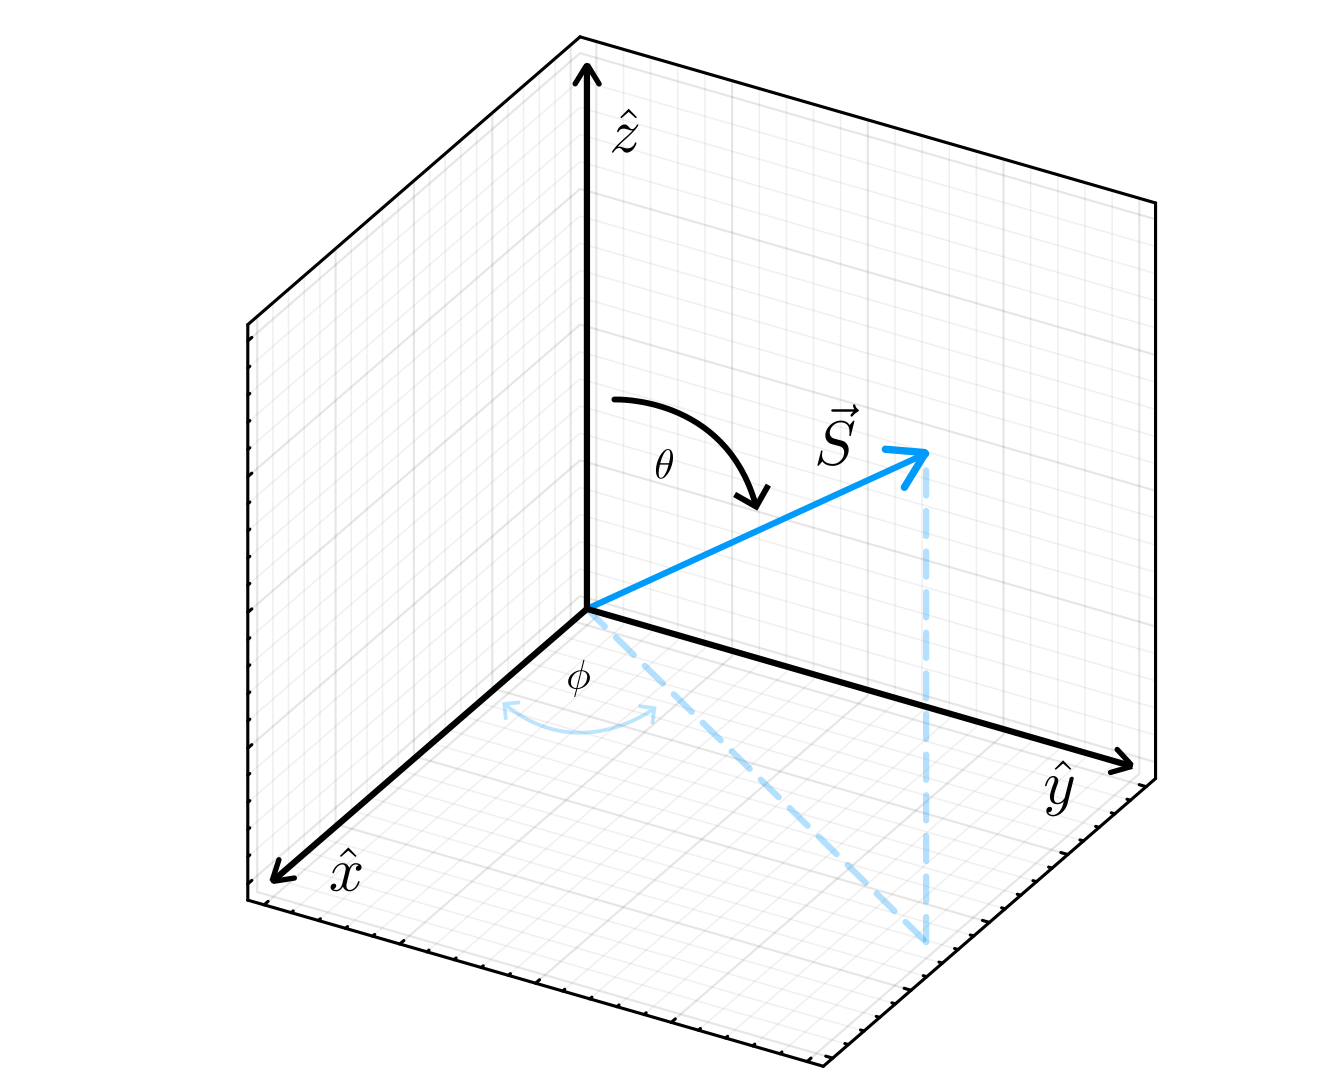
\includegraphics[width=0.5\textwidth]{appendix/rotation.png}
    \end{subfigure}
    \caption{Rotating the quantization axis}
\end{figure}
%%% FIG %%%
\FloatBarrier \!\!\!\!\!\!\!\!\!\!\!

This can be achieved by rotating the system by an angle of $\theta$ about the axis $\hat{n} = \hat{z} \cross \vec{S} =  (-\sin\phi, \cos\phi, 0)$. For a spin-1/2 particle, the rotation matrix is given as follows.
\begin{equation}
    R_{\vec{n}}(\alpha) = \exp{-\frac{\alpha}{2}\vec{n}\cdot\vec{\sigma}} = \mathbb{I}\cos\frac{\alpha}{2} + i (\hat{n}\cdot \vec{\sigma})\sin\frac{\alpha}{2}
\end{equation}
For our choice of rotation axis, this gives us the following matrix which is exactly what we found earlier in Eq. \eqref{eq:rot}!
\begin{equation}
    U = \begin{pmatrix}
        \cos\frac{\alpha}{2} + in_z\sin\frac{\alpha}{2} & i\sin\frac{\alpha}{2}(n_x - in_y) \\ 
        i\sin\frac{\alpha}{2}(n_x + in_y) & \cos\frac{\alpha}{2} - in_z\sin\frac{\alpha}{2}
    \end{pmatrix} =
    \begin{pmatrix}
        \cos\frac{\theta}{2} & -\sin\frac{\theta}{2}e^{-i\phi} \\ 
        \sin\frac{\theta}{2}e^{i\phi} & \cos\frac{\theta}{2}
    \end{pmatrix}
\end{equation}

Similarly, let us now consider the same hamiltonian in Eq. \ref{eq:spin-half} for a spin-1 particle.

\begin{equation}\label{eq:spin-one}
    H = \vec{S} \cdot \vec{J} = \begin{pmatrix}
        \cos\theta & \frac{1}{\sqrt{2}}\sin\theta e^{-i\phi} & 0 \\
        \frac{1}{\sqrt{2}}\sin\theta e^{i\phi} & 0 & \frac{1}{\sqrt{2}}\sin\theta e^{-i\phi} \\ 
        0 & \frac{1}{\sqrt{2}}\sin\theta e^{i\phi} & -\cos\theta
    \end{pmatrix}
\end{equation}

where $\vec{J}$ are the spin-1 matrices. The rotation matrix can then be written as follows\cite{Curtright_2014}.
\begin{equation}
    R_{\vec{n}}(\alpha) = \exp{-i\alpha \hat{n}\cdot\vec{J}} = \mathbb{I} + i\hat{n}\cdot\vec{J}\sin\alpha + (\hat{n}\cdot\vec{J})^2 (\cos\alpha - 1)
\end{equation}
Expanding this for our choice of rotation angle and axis, we obtain:
\begin{equation}
    U = \begin{pmatrix}
        \cos^2\frac{\theta}{2} & -\frac{1}{\sqrt{2}}\sin\theta e^{-i\phi} & \sin^2\frac{\theta}{2} e^{-2i\phi} \\
        \frac{1}{\sqrt{2}}\sin\theta e^{i\phi} & \cos\theta &-\frac{1}{\sqrt{2}}\sin\theta e^{-i\phi}\\
        \sin^2\frac{\theta}{2}e^{2i\phi} & \frac{1}{\sqrt{2}}\sin\theta e^{i\phi} & \cos^2\frac{\theta}{2}
    \end{pmatrix}
\end{equation}

It can be easily checked that this matrix does indeed diagonalize the hamiltonian in Eq. \eqref{eq:spin-one}. Thus, in general, such a hamiltonian is diagonalized by the rotation matrix that aligns the quantization axis to $\vec{S}$. This nice structure emerges due to the relation between the group that governs spin transformations, $SU(2)$, and the group that governs rotations in euclidean space, $SO(3)$\cite{palash2019}.